\section{The five-cell rule of Molofsky \emph{et al.}}
\label{app:molofsky}

\textit{Rule and closure.} The synchronous square-lattice rule of
Ref.~\cite{molofsky1999} assigns a site the state 1 with probability $p_n$,
where $n$ counts state-1 sites in its von Neumann neighborhood including
itself. Here $p_0=0$, $p_5=1$, $p_3=1-p_2$, and $p_4=1-p_1$.
Equivalently, a site with $j$ disagreeing neighbors flips with probability
$w(j)=p_j$. For $0<p_1,p_2<1$, every nonuniform configuration permits a
flip, giving exactly two absorbing configurations. The voter point is
$(p_1,p_2)=(1/5,2/5)$, where a site copies one of these five cells uniformly.

Write $w(j)=j/5+g(j)$, with
$g=(0,\delta_1,\delta_2,-\delta_2,-\delta_1)$ and
$(\delta_1,\delta_2)=(p_1-1/5,p_2-2/5)$. The voter dual consists of five
coalescing walks, each staying or moving to any nearest neighbor with
probability $1/5$. Averaging over $10^7$ recorded walk realizations at each
cutoff gives the finite-time reaction function
\begin{equation}
 \begin{gathered}
 f_T(u)=u(1-u)(1-2u)[a+c\,u(1-u)],
 \\
 c=P_5(T)(10\delta_2-5\delta_1),
 \end{gathered}
 \label{eq:fmol}
\end{equation}
where $a=\delta_1a_1(T)+\delta_2a_2(T)$ and $P_5$ is the probability that
all five lineages remain distinct. The coefficients $a_1,a_2$ include all
lineage patterns. Within the constant-diffusion scalar closure,
$f_T'(0)=a$, $f_T'(1/2)=-(a+c/4)/2$, and
$\int_0^{1/2}f_T(u)\,\ds u=(6a+c)/192$.
For $c>0$, the sector $-c/4<a<0$ is bistable, and its stationary front lies
at $a=-c/6$.

Table~\ref{tab:molofsky} and Fig.~\ref{fig:molofsky}(a,b) show the narrowing
of this sector with cutoff. The conditional probability
$\Pr(K\ge5\mid K\ge3)$, where $K$ is the surviving lineage count, is
smaller for the five-cell neighborhood than for the nine-cell Moore
neighborhood by factors 10.5, 17.2, 28.6, and 45.3 at
$T=16,64,1024,65536$. This comparison concerns the weight of higher-degree
contributions among patterns that can contribute to the drift. Ref.~\cite{molofsky1999}
found that isolated seeds can nucleate expanding patches in the spatial
model and did not observe the multiple-outcome regime of its mean-field map.

\begin{table}
\caption{Finite-time closure for the five-cell rule. Angles in degrees
are measured from the $+\delta_1$ axis. The columns give the absorbing-state
stability threshold, stationary-front condition, active-state stability
threshold, and sector width of the deterministic closure. The $10^7$
walk realizations give bootstrap standard errors below $0.05^\circ$ for
each angle.}
\label{tab:molofsky}
\begin{ruledtabular}
\begin{tabular}{rrrrrr}
$T$ & $P_5/P_{\ge3}$ & $\theta_a$ & $\theta_f$ & $\theta_{1/2}$ & width\\
\hline
16 & 0.0664 & 104.34 & 107.28 & 108.77 & 4.43\\
64 & 0.0253 & 105.32 & 106.60 & 107.25 & 1.92\\
256 & 0.011 & 105.73 & 106.32 & 106.62 & 0.90\\
1024 & 0.00520 & 105.93 & 106.23 & 106.38 & 0.45\\
4096 & 0.0027 & 106.03 & 106.19 & 106.27 & 0.24\\
65536 & 0.000784 & 106.09 & 106.14 & 106.17 & 0.07\\
\end{tabular}
\end{ruledtabular}
\end{table}

\textit{Expansion and interior decay.} We simulated the cuts $p_2=0.45$
and $0.50$ using random active strips, bulk random starts, $2\times2$ seeds,
and active disks. The fine strip scan uses $L_x=2048$, $L_y=4096$,
$T=10^5$, and four runs per point, supplemented by two runs per point at
$L_x=4096$. Profiles are smoothed over 32 rows. We measure half the slope
of the width using either a fixed half-reference threshold, half the
contemporaneous central activity, or the integrated activity divided by
the contemporaneous central activity. Fits retain records with fixed-threshold
width between $0.1L_y$ and $0.9L_y$ and central activity above 60\% of its
reference at $t=10^3$.

The mean normalized central activity decreases by at most 0.03 between
$t=3\times10^4$ and $10^5$ at three $L_x=2048$ points on each cut.
Their adaptive-width slopes are all positive. Equal-weight linear fits to
these three group means, using records from $t=2000$, extrapolate to zero
at $p_1^{\rm ext}=0.185345$ and 0.170569. Changing the fit start to
$t=30000$ and using the three width estimators gives the ranges in
Table~\ref{tab:molsim}. These are finite-window estimates of expansion onset.
The fitted adaptive branch has no negative-velocity point with a comparably
persistent interior to bracket its zero.

At $(p_2,p_1)=(0.45,0.18535)$, the normalized interior activity falls
from 0.781 to 0.705 between $3\times10^4$ and $10^5$. Its adaptive slope
changes from $+0.000216$ to $-0.000829$ when the fit start changes from
2000 to 30000. At $(0.50,0.17057)$ the corresponding activity falls from
0.818 to 0.754, and the slopes are $+0.000036$ and $-0.000057$.
These contracting profiles combine edge motion and interior decay.
The extrapolated onset directions are approximately $106.3^\circ$--$106.4^\circ$,
close to the large-cutoff closure and the chord from the voter point to
$(0.024,1)$ in Ref.~\cite{molofsky1999}. Their precision is limited by
relaxation and estimator choice.

\begin{table}
\caption{Five-cell simulations. The zero is extrapolated from the three
positive adaptive-width slopes satisfying the stated interior-drift criterion.
The range varies the width estimator and fit start and gives a sensitivity
assessment. Each run reaches $10^5$ steps. The final rows give bulk interface
densities at the stated actual probabilities and observation horizons.}
\label{tab:molsim}
\begin{ruledtabular}
\begin{tabular}{lll}
 & $p_2=0.45$ & $p_2=0.50$\\
\hline
$p_1^{\rm ext}$ & 0.185345 & 0.170569\\
Range lower bound & 0.185345 & 0.170569\\
Range upper bound & 0.185397 & 0.170607\\
Smallest fitted $p_1$ & 0.185400 & 0.170620\\
$p_1$ of bulk sample & 0.185400 & 0.170620\\
$L$ & 2048 & 2048\\
Bulk horizon & $1.2\times10^6$ & $3\times10^5$\\
Late $\rho$ & $0.188(1)$ & $\approx0.20$\\
\end{tabular}
\end{ruledtabular}
\end{table}

\begin{figure*}
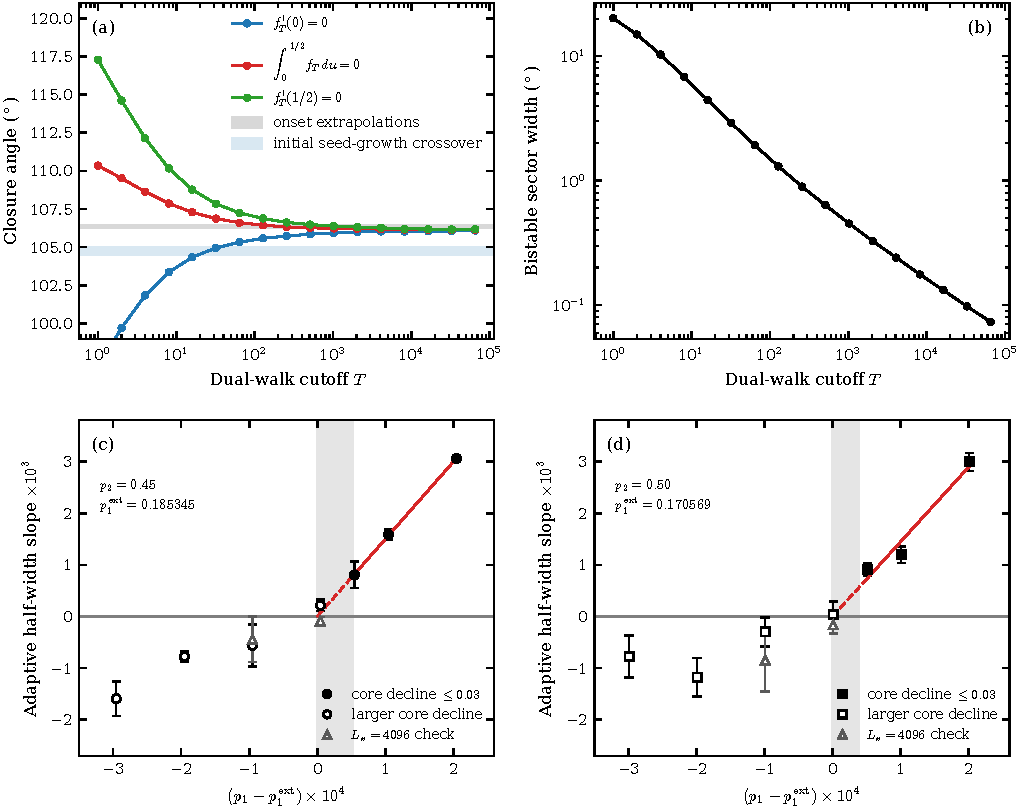
\includegraphics[width=\textwidth]{figs/fig_molofsky}
\caption{Five-cell closure and finite-time strip dynamics.
(a) Closure threshold angles versus dual-walk cutoff. Gray shading spans the
extrapolated onset angles from the two cuts, three width estimators, and two
fit windows. Blue shading marks the approximate initial seed-growth crossover
reported in the sampled ensembles. (b) Angular width of the closure's bistable
sector. (c,d) Half-slopes of the adaptive strip width from records with
$t\ge2000$ on the two cuts, with one standard error over runs. Filled points
have an ensemble-mean normalized interior decline of at most 0.03 between
$3\times10^4$ and $10^5$; open points show stronger interior decay.
Triangles are the two-run $L_x=4096$ checks; circles and squares are four-run
$L_x=2048$ groups. Solid segments fit the three filled $L_x=2048$ points,
and dashed segments extrapolate to zero. Gray bands give the corresponding
estimator/window ranges. The horizontal origin is the displayed early-window
adaptive extrapolation $p_1^{\rm ext}$.}
\label{fig:molofsky}
\end{figure*}

\textit{Seeds, bulk relaxation, and absorption.} The mean population of
$2\times2$ seeds initially decreases up to approximately $p_1=0.187$--0.188
on the first cut and 0.173--0.174 on the second. At $(p_2,p_1)=(0.45,0.186)$,
93 of 20000 seeds survive to $10^4$ steps. Active disks have finite-time
half-survival radii $R_{1/2}(2\times10^4)$ with products
$R_{1/2}v=0.1595$--0.1846 in four sampled cases, comparable with the voter
diffusion coefficient $1/5$. A fifth case gives $R_{1/2}>28$.
All recorded escape counts are zero. The ensembles stop at 100 survivors
or 400 replicas for disks and 300 survivors or 20000 replicas for small
seeds. Their endpoint proportions describe these adaptive samples.

At $p_2=0.45$, bulk runs at $p_1=0.18540$ have late mean
$\rho=0.188(1)$ for $L=2048$ through $1.2\times10^6$ and $0.190(1)$ for
$L=4096$ through $6\times10^5$. Nearby $p_1=0.18538$ and 0.18539 runs show
continuing drift or broad run-to-run variation. Logarithmic vanishing,
a small power, and a finite jump can describe the sampled density curve
when its boundary location is varied. This leaves the transition order open.

At the earlier reference values $p_1=0.18535$ and 0.17057, the all-run
restricted mean absorption times $\langle\min(T_{\rm abs},10^6)\rangle$
are $2.413\times10^5$ and $2.321\times10^5$ at $L=256$, increasing to
$5.942\times10^5$ and $8.539\times10^5$ at $L=512$. Each ensemble contains
four runs. All four absorb at $L=256$, whereas three absorb at $L=512$;
the remaining run contributes its full observation horizon. The density
relaxes through coarsening, and these runs resolve no persistent active
slab retreating as a coherent phase.

The observations place expansion onset, early seed suppression, and loss
of an apparent bulk plateau on different finite-time scales. These
observables offer tests of the closure, whose spinodal thresholds refer
to the deterministic reaction equation. The simulations resolve neither
those spinodals nor a metastable active branch for the five-cell rule.
A closure calibrated only to expansion onset therefore does not explain
the stronger coexistence signatures of the D\&N model.
